\documentclass[10pt,a4paper]{article}
\usepackage{tikz-feynman}
\tikzfeynmanset{compat=1.0.0}
\begin{document}

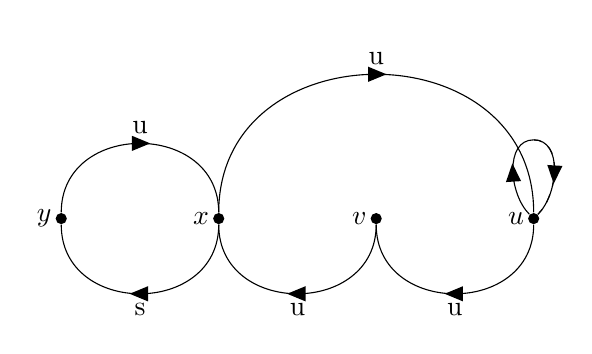
\begin{tikzpicture}
  \begin{feynman}
    % \node [inner sep=0.02cm](u) at (0,0) {\textbullet};
    % \node (v) at (2,0) {\textbullet};
    % \node (x) at (4,0) {\textbullet};
    % \node (y) at (6,0) {\textbullet};
    \node [inner sep=0.05cm, circle, fill](u) at (6,0) {};
    \node [inner sep=0.05cm, circle, fill](v) at (4,0) {};
    \node [inner sep=0.05cm, circle, fill](x) at (2,0) {};
    \node [inner sep=0.05cm, circle, fill](y) at (0,0) {};

    \draw (u) node[left] {$u$};
    \draw (v) node[left] {$v$};
    \draw (x) node[left] {$x$};
    \draw (y) node[left] {$y$};

    
    % \node[above = 1cm of u] (uu);
    \vertex[above = 1cm of u] (uu);
    \vertex[above = 1cm of v] (vv);
    \vertex[above = 1cm of x] (xx);
    \vertex[above = 1cm of y] (yy);
 % input nodes position and text
\diagram*{
  {[edges={fermion, half left}]
    (u) --[edge label=u] (v),
    (v) --[edge label=u] (x), 
    (x) --[edge label=s] (y),
    (x) --[edge label=u] (u),
    (y) --[edge label=u] (x),
  },

  % self-connected quark loop
  {[edges={fermion}]
    (u)  -- [out=135,in=180] (uu) --[scalar,out=0,in=45] (u)
  },
};
  \end{feynman}
\end{tikzpicture}


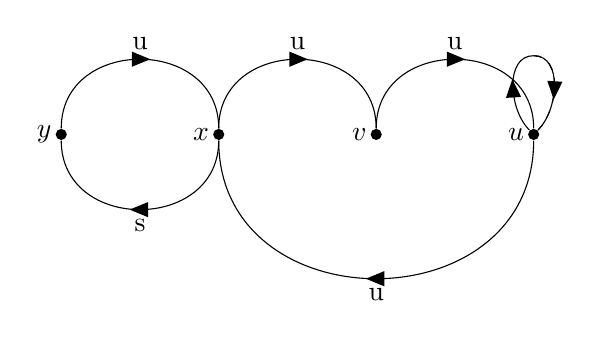
\begin{tikzpicture}
  \begin{feynman}
    % \node [inner sep=0.02cm](u) at (0,0) {\textbullet};
    % \node (v) at (2,0) {\textbullet};
    % \node (x) at (4,0) {\textbullet};
    % \node (y) at (6,0) {\textbullet};
    \node [inner sep=0.05cm, circle, fill](u) at (6,0) {};
    \node [inner sep=0.05cm, circle, fill](v) at (4,0) {};
    \node [inner sep=0.05cm, circle, fill](x) at (2,0) {};
    \node [inner sep=0.05cm, circle, fill](y) at (0,0) {};

    \draw (u) node[left] {$u$};
    \draw (v) node[left] {$v$};
    \draw (x) node[left] {$x$};
    \draw (y) node[left] {$y$};

    
    % \node[above = 1cm of u] (uu);
    \vertex[above = 1cm of u] (uu);
    \vertex[above = 1cm of v] (vv);
    \vertex[above = 1cm of x] (xx);
    \vertex[above = 1cm of y] (yy);
 % input nodes position and text
\diagram*{
  {[edges={fermion, half left}]
    (u) --[edge label=u] (x),
    (v) --[edge label=u] (u), 
    (x) --[edge label=s] (y),
    (x) --[edge label=u] (v),
    (y) --[edge label=u] (x),
  },

  % self-connected quark loop
  {[edges={fermion}]
    (u)  -- [out=135,in=180] (uu) --[scalar,out=0,in=45] (u)
  },
};
  \end{feynman}
\end{tikzpicture}

\end{document}


